\section*{Process description}


Nitroma's process for the nitration of toluene and subsequent reduction and hydrogenation of nitrotoluenes is unique in both its continuous operating mode and the production of three different substituted aromatic amines.  \Cref{fig:BFD-ES} is a simplified process flow diagram of the process.
\begin{wrapfigure}{l}{0.55\linewidth}
    \centering
    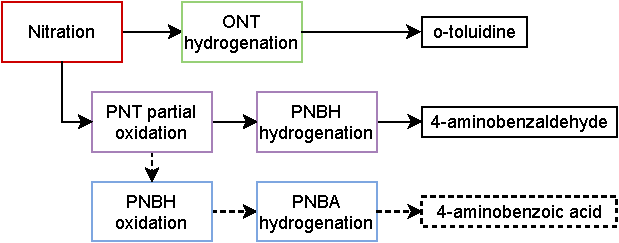
\includegraphics[width=0.8\linewidth]{chapters/0-executive-summary/figures/BFD_nitroma-Page-3.pdf}
    \caption{Simplified synthesis route for Nitroma's process}
    \label{fig:BFD-ES}
\end{wrapfigure}
Firstly, the nitration of toluene with 70\% aqueous nitric acid is carried out in a shell-and-tube heat exchanger reactor packed with H-mordenite catalyst. Solid acid catalysts were preferred over the traditional mixed-acid synthesis due to environmental, safety and performance advantages. Zeolites indeed alleviate the need for costly and energy intensive regeneration of corrosive sulphuric acid, as well as preventing the emission of toxic and global warming potential nitrogen oxides. Heterogeneous catalysis is also attractive from an economical point of view since it favours the more economically desirable \para-nitrotoluene (PNT) isomer. The nitration reactor effluent is fed to a decanter to separate the aqueous nitric acid from the organic phase. Following water evaporation in a distillation column, nitric acid is recycled back into the nitration reactor at a \SI{94}{mol\percent} purity. Meanwhile, the organic phase is sent to a distillation column to recycle unreacted toluene to the nitration reactor. The nitrotoluenes are sent to a second distillation column to separate the more volatile o-nitrotoluene (ONT) from m-nitrotoluene (MNT) and PNT. The large difference in the PNT and MNT melting points is exploited in a mixed-suspension mixed-product removal crystalliser.




